%Input preamble
%Style
\documentclass[12pt]{article}
\usepackage[top=1in, bottom=1in, left=1in, right=1in]{geometry}
\parindent 22pt
\usepackage{fancyhdr}

%Packages
\usepackage{adjustbox}
\usepackage{amsmath}
\usepackage{amsfonts}
\usepackage{amssymb}
\usepackage{bm}
\usepackage[table]{xcolor}
\usepackage{tabu}
\usepackage{color,soul}
\usepackage{makecell}
\usepackage{longtable}
\usepackage{multirow}
\usepackage[normalem]{ulem}
\usepackage{etoolbox}
\usepackage{graphicx}
\usepackage{tabularx}
\usepackage{ragged2e}
\usepackage{booktabs}
\usepackage{caption}
\usepackage{fixltx2e}
\usepackage[para, flushleft]{threeparttablex}
\usepackage[capposition=top,objectset=centering]{floatrow}
\usepackage{subcaption}
\usepackage{pdfpages}
\usepackage{pdflscape}
\usepackage{natbib}
\usepackage{bibunits}
\definecolor{maroon}{HTML}{990012}
\usepackage[colorlinks=true,linkcolor=maroon,citecolor=maroon,urlcolor=maroon,anchorcolor=maroon]{hyperref}
\usepackage{marvosym}
\usepackage{makeidx}
\usepackage{tikz}
\usetikzlibrary{shapes}
\usepackage{setspace}
\usepackage{enumerate}
\usepackage{rotating}
\usepackage{tocloft}
\usepackage{epstopdf}
\usepackage[titletoc]{appendix}
\usepackage{framed}
\usepackage{comment}
\usepackage{xr}
\usepackage{titlesec}
\usepackage{footnote}
\usepackage{longtable}
\newlength{\tablewidth}
\setlength{\tablewidth}{9.3in}
\setcounter{secnumdepth}{4}

\titleformat{\paragraph}
{\normalfont\normalsize\bfseries}{\theparagraph}{1em}{}
\titlespacing*{\paragraph}
{0pt}{3.25ex plus 1ex minus .2ex}{1.5ex plus .2ex}
\makeatletter
\pretocmd\start@align
{%
  \let\everycr\CT@everycr
  \CT@start
}{}{}
\apptocmd{\endalign}{\CT@end}{}{}
\makeatother
%Watermark
\usepackage[printwatermark]{xwatermark}
\usepackage{lipsum}
\definecolor{lightgray}{RGB}{220,220,220}
%\newwatermark[allpages,color=lightgray,angle=45,scale=3,xpos=0,ypos=0]{Preliminary Draft}

%Further subsection level
\usepackage{titlesec}
\setcounter{secnumdepth}{4}
\titleformat{\paragraph}
{\normalfont\normalsize\bfseries}{\theparagraph}{1em}{}
\titlespacing*{\paragraph}
{0pt}{3.25ex plus 1ex minus .2ex}{1.5ex plus .2ex}

\setcounter{secnumdepth}{5}
\titleformat{\subparagraph}
{\normalfont\normalsize\bfseries}{\thesubparagraph}{1em}{}
\titlespacing*{\subparagraph}
{0pt}{3.25ex plus 1ex minus .2ex}{1.5ex plus .2ex}

%Functions
\DeclareMathOperator{\cov}{Cov}
\DeclareMathOperator{\corr}{Corr}
\DeclareMathOperator{\var}{Var}
\DeclareMathOperator{\plim}{plim}
\DeclareMathOperator*{\argmin}{arg\,min}
\DeclareMathOperator*{\argmax}{arg\,max}

%Math Environments
\newtheorem{theorem}{Theorem}
\newtheorem{claim}{Claim}
\newtheorem{condition}{Condition}
\renewcommand\thecondition{C--\arabic{condition}}
\newtheorem{algorithm}{Algorithm}
\newtheorem{assumption}{Assumption}
\renewcommand\theassumption{A--\arabic{assumption}}
\newtheorem{remark}{Remark}
\renewcommand\theremark{R--\arabic{remark}}
\newtheorem{definition}[theorem]{Definition}
\newtheorem{hypothesis}[theorem]{Hypothesis}
\newtheorem{property}[theorem]{Property}
\newtheorem{example}[theorem]{Example}
\newtheorem{result}[theorem]{Result}
\newenvironment{proof}{\textbf{Proof:}}{$\bullet$}

%Commands
\newcommand\independent{\protect\mathpalette{\protect\independenT}{\perp}}
\def\independenT#1#2{\mathrel{\rlap{$#1#2$}\mkern2mu{#1#2}}}
\newcommand{\overbar}[1]{\mkern 1.5mu\overline{\mkern-1.5mu#1\mkern-1.5mu}\mkern 1.5mu}
\newcommand{\equald}{\ensuremath{\overset{d}{=}}}
\captionsetup[table]{skip=10pt}
%\makeindex

\setlength\parindent{0pt}
\setlength{\parskip}{10pt}

\newcolumntype{L}[1]{>{\raggedright\let\newline\\\arraybackslash\hspace{0pt}}m{#1}}
\newcolumntype{C}[1]{>{\centering\let\newline\\\arraybackslash\hspace{0pt}}m{#1}}
\newcolumntype{R}[1]{>{\raggedleft\let\newline\\\arraybackslash\hspace{0pt}}m{#1}}



%Logo
%\AddToShipoutPictureBG{%
%  \AtPageUpperLeft{\raisebox{-\height}{
\includegraphics[width=1.5cm]{uchicago.png}}}
%}

\newcolumntype{L}[1]{>{\raggedright\let\newline\\\arraybackslash\hspace{0pt}}m{#1}}
\newcolumntype{C}[1]{>{\centering\let\newline\\\arraybackslash\hspace{0pt}}m{#1}}
\newcolumntype{R}[1]{>{\raggedleft\let\newline\\\arraybackslash\hspace{0pt}}m{#1}}

\newcommand{\mr}{\multirow}
\newcommand{\mc}{\multicolumn}

%\newcommand{\comment}[1]{}

%Other parameters
\newcommand{\noutcomes}{95}
\newcommand{\noutcomesexpp}{357}
\newcommand{\noutcomesexpm}{343}
\newcommand{\noutcomesexpf}{355}
\newcommand{\treatsubsabc}{$75\%$}
\newcommand{\treatsubscarec}{$74\%$}
\newcommand{\treatsubscaref}{$63\%$}

%Counts
%Males
\newcommand{\positivem}{$78\%$}
\newcommand{\positivesm}{$29\%$}

%Females
\newcommand{\positivef}{$78\%$}
\newcommand{\positivesf}{$31\%$}

%Counts, control substitution
%Males
\newcommand{\positivecsnm}{$47\%$}
\newcommand{\positivescsnm}{$15\%$}

\newcommand{\positivecsam}{$79\%$}
\newcommand{\positivescsam}{$29\%$}

%Females
%% no alternative
\newcommand{\positivecsnf}{$84\%$}
\newcommand{\positivescsnf}{$55\%$}

%% alternative
\newcommand{\positivecsaf}{$79\%$}
\newcommand{\positivescsaf}{$33\%$}

%Pooled

%Effects
%Males

%Females
\newcommand{\empf}{$8$}
\newcommand{\yearsedf}{$1.7$}



%Pooled

%CBA
%IRR
%Males
\newcommand{\irrm}{$15\%$}
\newcommand{\irrsem}{$5\%$}

%Females
\newcommand{\irrf}{$9\%$}
\newcommand{\irrsef}{$7\%$}

%Pooled
\newcommand{\irrp}{$13\%$}
\newcommand{\irrsep}{$5\%$}

%BC
%Males
\newcommand{\bcm}{$11.24$}
\newcommand{\bcsem}{$4.60$}

%Females
\newcommand{\bcf}{$2.35$}
\newcommand{\bcsef}{$1.09$}

%Pooled
\newcommand{\bcp}{$5.63$}
\newcommand{\bcsep}{$2.15$}

%NPV streams
%Pooled
\newcommand{\parincomenpvp}{$\$119,346$}
\usepackage[stable]{footmisc}

\newcommand*\leftright[2]{%
  \leavevmode
  \rlap{#1}%
  \hspace{0.5\linewidth}%
  #2}

\newcommand{\orth}{\ensuremath{\perp\!\!\!\perp}}%
\newcommand{\indep}{\orth}%
\newcommand{\notorth}{\ensuremath{\perp\!\!\!\!\!\!\diagup\!\!\!\!\!\!\perp}}%
\newcommand{\notindep}{\notorth}

\renewcommand{\theequation}{R.\arabic{equation}}

\externaldocument{abc_comprehensivecba_appendix-pub}
\externaldocument{abc_comprehensivecba_revised}
\doublespacing

\begin{document}

\singlespacing
\begin{titlepage}
\newgeometry{top=.8in, bottom=.8in, left=.8in, right=.8in}

\title{\Large \textbf{Second-round Responses to the Editor and the Referees \\ Quantifying the Life-cycle \\ Benefits of an Influential Early Childhood Program}}

\author{
Jorge Luis Garc\'{i}a\\
John E. Walker  Department of Economics\\
Clemson University \\
Social Science Research Institute \\
Duke University \\  \and
James J. Heckman \\
American Bar Foundation \\
Center for the Economics of Human Development \\
The University of Chicago \and
Duncan Ermini Leaf \\
Leonard D. Schaeffer Center \\  for Health Policy and Economics\\
University of Southern California \and
Mar\'{i}a Jos\'{e} Prados \\
Dornsife Center for \\ Economic and Social Research\\
University of Southern California}
\date{First Draft: January 5 , 2018\\ This Draft: \today}

\maketitle
\thispagestyle{empty}
\end{titlepage}

\restoregeometry
\doublespacing

\noindent We thank you all for your second round of thoughtful comments which have led to substantial improvement in the paper. Itemized responses to each of the questions posed follow.

\section*{Comments of the Editor}

\noindent \textbf{Editor, Comment 1. Please send in what you want me and the referees to consider to be the final version. When you send in your revision, make sure to also include a reply to me as well as to the remaining referee, explaining what you did with the comments you received.} 

\noindent \textit{Response.} We are submitting what we consider our final version. Responses to your questions and the referees' questions follow. 

\noindent \textbf{Editor, Comment 2. Keep in mind that this is, ultimately, your paper. I very much hope that we can get by with one last round of revisions at this point. I believe this is in our mutual interest. This, obviously, depends much on you providing a dedicated revision. It should not exceed the current length by more than three pages, i.e. not exceed 42 pages, including the references.}

\noindent \textit{Response.} We hope so too, and think of this as the final version of our project. We have complied to the page limit that you indicated.

\noindent \textbf{Editor, Comment 3. I assume that the material following the references is meant to be an online appendix: please clearly indicate (and confirm) that this is so.}

\noindent \textit{Response.} Yes. The material after the references is for online consultation and we would appreciate if it can me posted as an online appendix.

\noindent \textbf{Editor, Comment 4. At this point, please provide the appropriate documentation along with your resubmission.}

\noindent \textit{Response.} The front page of the paper has a link to the online repository containing the code for each and all of our computations, together with the corresponding replication instructions. We cannot post the data because it is not open access, but we can facilitate any person interested in replicating our computations the adequate contacts to request access to the data. Once access to the data is provided, we can provide help with replicating any of our computations.

\section*{Comments of Reviewer 1}

\noindent \textbf{Referee 1, Comment 1. None of the children came from Raleigh, NC. All lived within 8 miles of the Frank Porter Graham Child Development Center in Chapel Hill, NC where the early education program was provided. All lived inside Orange County and were born in Memorial Hospital. (These are well-reported facts.)}

\noindent \textit{Response.} We appreciate this clarification and have modified the first paragraph of Section~\ref{section:background} accordingly.

\textit{\textbf{[JLG: I spoke to Peg Burchinal and to Anna (who visited the archives of the Frank Porter Graham Center) and they maintain that the most that they know about the birthplace of the children is that it was in the Research Triangle Area. None of them knew the ``well-reported fact'' that all children were born in Memorial Hospital, although Peg think that it is likely that most of the children did. In any event, I propose the following minor modification to the first paragraph of Section~\ref{section:background} because I don't think it's worth it to fight off the referee on this minor detail. ``The Carolina Abecedarian Project and the Carolina Approach to Responsive Education (ABC/CARE) were enriched childcare programs that targeted the early years of disadvantaged, predominately African-American children in the area of Chapel Hill, North Carolina. Appendix A describes these programs in detail. We summarize their main features here.'']}}

\noindent \textbf{Referee 1, Comment 2. It is stated that the program ``provided health screenings to treatment-group members with costs of medication borne by parents.'' This is wrong. All children in all treatment groups received free health care (much more than ``screening'') conforming the American Academy of Pediatrics recommended schedule, and this included covering costs of medication, except if the child's family had existing health care coverage that could appropriately assume costs.}

\noindent \textit{Response.} Thanks for this comment. We have further investigated the health screenings and have revised the second paragraph of Section~\ref{section:background}.

\textit{\textbf{[JLG: There seems to be conflicting information between my notes of our meeting with Peg Burchinal in Chicago a long time ago and what the referee states. It was in the meeting what we had back then with Peg that she noted that the costs of medication were borne by the parents. The battery of references by Campbell, Ramey, and etc. are not careful when describing the health component of the program. I further communicated with Peg and the issue of the costs is not clear. I propose that we compromise and write the last sentence of the second paragraph of Section~\ref{section:background} as follows. ``All treatment children received medical check-ups that conformed with the American Academy. Parents were notified if children had medical issues. The first cohort of the ABC control-group received similar services \citep{Campbell_Conti_etal_2014_EarlyChildhoodInvestments,Henderson-et-al_1982_NEJoM}.'']}}

\noindent \textbf{Referee 1, Comment 3. The second phase of the study is described as consisting of ``home visits from ages 5 to 8." This is wrong. The actual phase 2 was a structured ``home and school resource program'' that operated from kindergarten through the entrance into third grade. The program had home visits, school visits, and summer day programs. This is much more than a home visiting program.}

\noindent \textit{Response.} We appreciate this comment and acknowledge that our focus on the first phase of the program lead us to a brief and imprecise description of the second phase of the program. We have modified the description of the second phase of the program in the third paragraph of Section~\ref{section:background}.

\textit{\textbf{[JLG: I think that here the referee is right. I did not pay enough attention to the description of the second phase of the program and what we wrote is incomplete. Peg recommended some sources and I propose that we amend the third paragraph of Section~\ref{section:background} as follows. (Note that Peg insists that the summer school that the referee mentions was not part of the second phase. But, again, I think that that really becomes a minor detail. The amendment that I propose should take care of the main concern that she has.) ``The design and implementation of ABC and CARE were very similar. Both had two phases, the first of which lasted from birth until age 5. In this phase, children were randomly assigned to treatment. The second phase of the study took place for the first three years of public school and supported children's academic development. It enhanced parental involvement in the education of the children. A home visit took place every two weeks and provided parents home activities to complement the skills taught at school. The visitor facilitated communication between the teachers and the parents \citep{Campbell_Ramey_1995_AERJ}. Children were assigned to this treatment through a second-stage randomization. The first phase of CARE, from birth until age 5, had an additional treatment arm of home visits designed to improve home environments.'']}}  

\noindent \textbf{Referee 1, Comment 4. Authors state ``data were collected annually on cognitive and social-emotional skills…'' This simplifies incorrectly. The common data collection (there were minor variations not worthy of mention for this paper) were at 6 month intervals through age 5 (60 mos.), then at age 6 and next on to the ages 8, 12, 15, and 30 already mentioned in the next sentence. Since this is not ``annual" the sentence should be corrected - and there are not 7 year old data. This is minor, but an example for careless characterization of the study, given the tremendous emphasis on details about computing social efficiency overall. Another example of carelessness in description of methodology is the statement that additional information was collected ``from a physician-administered medical survey, when the subjects were in their mid-30s.'' In fact, there was an in-person set of assessments, included collection of bio specimens and measurements. This is not a survey. Statement should be corrected to correspond to what occurred, especially since health outcomes based on this one-time assessment are incorporated in the forecasting models.} 

\noindent \textit{Response.} This comment is very useful because we were incorrectly simplifying the data collection. We have modified the last paragraph of Section~\ref{section:background} accordingly.

\textit{\textbf{[JLG: As the referee herself says, we oversimplified here and we should probably avoid details. I propose the following modification to the las paragraph of Section~\ref{section:background}. ``For both programs, data were frequently collected on cognitive and socio-emotional skills, home environments, family structure, and family economic characteristics from birth until age 8. Further follow-ups were collected at ages 12, 15, 21, and 30. In addition, there is information from administrative criminal records, and from a full in-person medical assessment that included a survey and collection of bio specimens and measurements when the subjects were in their mid30s. Many control-group children in both ABC and CARE attended alternative formal childcare arrangements (75\% and 74\%, respectively).'']}} 

\noindent \textbf{Referee 1, Comment 5. I strongly recommend that the authors modify their simplification of the ABC/CARE intervention as mostly just free high-quality childcare for more than 9 hrs/day, 50 wks/yr is seriously misleading. At the very least, the authors should add several words that capture that this was ``an enriched, educationally focused child care center program'' or ``an early educational intervention in a high-quality child care center'' (which had a curriculum and active supervision of care providers and licensed teachers - informed by scientific knowledge at that time about how infants, toddlers, and young children learn. Why this is important is that many policymakers and economists may naively think that this is equal to subsidized child care in our country. This would be a misleading interpretation for what this paper shows - beyond demonstrating how to compute models of lifelong benefits. That is, this article serves two purposes: one is the proposal of how to calculate benefits from interventions and the other is the particular benefits of these two combined programs. The article needs to be informative and scientifically accurate on both purposes.}

\noindent \textit{Response.} We appreciate this point and have modified the second paragraph of Section~\ref{section:background} accordingly.

\textit{\textbf{[JLG: While this point feels mainly semantic, I propose that we slightly modify the second paragraph of Section~\ref{section:background} to the following. ``These programs went beyond regular care. They were high-quality, educationally-focused child care centers. Their goal was to enhance the life skills of disadvantaged children. They supported language, motor, and cognitive development as well as socio-emotional competencies considered crucial for school success including task orientation, the ability to communicate, independence, and pro-social behavior.11 They also provided free health screenings to treatment-group members with costs of medications borne by the parents.'']}}

\section*{Comments of Reviewer 2}

\noindent \textbf{Referee 2, Comment 1. [\ldots] Assumption~\ref{ass:contain} does not seem exactly right. For the $n$ group, $d = 0$ always in your sample which means that $\bm{X}_{k,a}^1$ is never observed. Yet, since Assumption~\ref{ass:contain} holds for $d \in \{ 0,1 \}$ it holds for $d = 1$ which says:} 

\begin{equation}
supp( \bm{Y}_{e,a}^1, \bm{X}^1_{e,a}, \bm{B}_e, \bm{\varepsilon}_{e,a} ) \subseteq supp( \bm{Y}_{e,a}^1, \bm{X}^1_{e,a}, \bm{B}_e, \bm{\varepsilon}_{e,a} ). \label{eq:ref1}
\end{equation}

\textbf{but since $\bm{X}_{k,a}^1$ is never observed, I don't think its support is relevant. it seems like it should be something like} 

\begin{equation}
supp( \bm{Y}_{e,a}^1, \bm{X}^1_{e,a}, \bm{B}_e, \bm{\varepsilon}_{e,a} ) \subseteq supp( \bm{Y}_{e,a}^0, \bm{X}^0_{e,a}, \bm{B}_e, \bm{\varepsilon}_{e,a} ).  \label{eq:ref2}
\end{equation}

\textbf{or perhaps more generally}

\begin{equation}
supp( \bm{Y}_{e,a}^1, \bm{X}^1_{e,a}, \bm{B}_e, \bm{\varepsilon}_{e,a} ) \subseteq supp( \bm{Y}_{e,a}^d, \bm{X}^d_{e,a}, \bm{B}_e, \bm{\varepsilon}_{e,a} ).  \label{eq:ref3}
\end{equation}

\noindent \textit{Response.} The statement of Assumption~\ref{ass:contain} in the main text is correct and comprehensive. While the referee is right that we do not observe $\bm{X}_{k,a}^1$ for $k = n$, the statement of the assumption is counterfactual. We require the non-experimental sample ($k = n$) to cover the support of the outputs and inputs in the experimental sample ($k = e$) so that when we estimate the production function in the non-experimental sample they are valid means of forecast in the experimental sample. 

It is hard to understand the point of the referee when using Equation~\eqref{eq:ref1} because he made a notational mistake as the right- and the left-hand side of the equations is the exact same. The equation that he wrote trivially holds and that is not what we assume.

Additionally, Equation~\eqref{eq:ref2} is not really a support condition of our interest: We are not trying to use the control-group in the experimental sample to forecast in the treatment-group in the experimental sample, which would seem the implication from what the referee writes. Similarly for what the referee writes in Equation~\eqref{eq:ref3}. Perhaps what the referee meant to write was 

\begin{equation}
supp( \bm{Y}_{e,a}^d, \bm{X}^d_{e,a}, \bm{B}_e, \bm{\varepsilon}_{e,a} ) \subseteq supp( \bm{Y}_{n,a}^0, \bm{X}^0_{n,a}, \bm{B}_n, \bm{\varepsilon}_{n,a} ).  \label{eq:ref4},
\end{equation}

which holds as a direct consequence of Assumption~\ref{ass:contain}.

\noindent \textbf{Referee 2, Comment 2. [\ldots] It feels that this is more complicated than it needs to be. For example, I don't understand why you need to distinguish between $\bm{\phi}_{k,a}^d \left( \cdot, \cdot \right) $ and $\bm{\varepsilon}_{k,a}^d$. You motivate this with the conditional mean $\Delta_a$ so if I focus on identifying that, one needs to identify}

\begin{equation}
\mathbb{E} \left[ \bm{Y}_{e,a}^d | \bm{B} \in \mathcal{B}_0 \right] = \int \mathbb{E} \left[ \bm{Y}_{e,a}^d | \bm{X}_{e,a} = x, \bm{B} \in \mathcal{B}_0 \right] G_{e,a}^d \left( \bm{x} \right)
\end{equation}

\textbf{where $G_{e,a}^d \left( \bm{x} \right)$, then since $G_{e,a}^1$ is presumably identified from the experimental sample it seems like you use two conditions. The first is that}

\begin{equation}
\mathbb{E} \left[  \bm{Y}_{e,a}^d | \bm{X}_{e,a}^d = \bm{x},  \bm{B} \in \mathcal{B}_0 \right] = \mathbb{E} \left[  \bm{Y}_{n,a}^0 | \bm{X}_{n,a}^0 = \bm{x},  \bm{B} \in \mathcal{B}_0 \right]  \label{eq:ref4}
\end{equation}

\textbf{which seems to be implied by Assumptions~\ref{ass:summary} to \ref{ass:exog}. The second is the support condition Assumption~\ref{ass:contain}. Why not presenting it this way? Am I missing something?}

\noindent \textit{Response.} First, the reason why we include $\bm{\varepsilon}_{k,a}^d$ in Assumption~\ref{ass:summary} is that we are stating invariance in the production function in Equation~\eqref{eq:outcome}. The components of this production function are both $\bm{\phi}_{k,a}^d \left( \cdot, \cdot \right) $ and $\bm{\varepsilon}_{k,a}^d$. Thus, for the production function to be invariant across treatment regimes and samples, we need to state and test invariance conditions for all of the components. We do not want to arbitrarily state invariance conditions on one element of the production function and not in the other, even when $\bm{\phi}_{k,a}^d \left( \cdot, \cdot \right) $ is our forecasting tool. Note also that including $\bm{\varepsilon}_{k,a}^d$ in the invariance assumption provides us with additional implications that we present tests for.

Second, Assumption~\ref{ass:summary} states and clarifies the economic concept that implies Equation~\eqref{eq:ref4}. We pose the assumption and derive the implications in Equations~\eqref{eq:suff1},~\eqref{eq:suff2}, and~\eqref{eq:nec},  which include Equations~\eqref{eq:ref4}. 

The analogous answer applies for the case of identifying distributions, as opposed to conditional means (as the referee points out).

\noindent \textbf{Referee 2, Comment 3. It seems like we need some assumption about $\bm{X}_{e,a}^d$. In general, if Assumptions~\ref{ass:summary} to \ref{ass:exog} hold but I want to identify $\mathbb{E} \left[ \bm{Y}_{e,a} | \bm{B} \in \mathcal{B}_0 \right]$ for $a^* < a$, I typically won't observe $\bm{X}_{e,a}^d$ in the data but if I can't observe $\bm{X}_{e,a}^d$ why is exogeneity useful? Thus it seems that for identification we need an additional assumption about identification of $\bm{X}_{e,a}^d$. It seems like essentially just assuming $G_{e,a}^d \left( \bm{x} \right)$ is identified in my example above.} 

\noindent \textit{Response.} It is true that observing $\bm{X}_{e,a}^d$ is necessary and crucial to our forecasting methodology. We do not pose that as an assumption but as part of our empirical procedure because it is the inputs of the production function are chosen by the researcher. \textbf{Step 3.} in Section~\ref{sec:forecasting} is precisely devoted to explain and justify the election of the inputs that we use. In sum, the inputs need to be observed in both the experimental and the non-experimental samples, satisfy common support, and be relevant in predicting the outcome of interest. Else, it would be impossible to form a forecast.

\section*{Comments of Reviewer 3}

\noindent \textbf{Referee 3, Comment 1. A key assumption is that the mapping between predictors and outcomes to be constant across children, parents, and grand-children, once you control for background variables. Can't this assumption be relaxed to allow for interactions between cohort and predictors/outcomes in a parametric/restrictive way? For example, I suppose you could allow for say a (e.g. linear) trend between cohort of birth and these variables. Can data be informative about how one would specify such a trend?}

\noindent \textit{Response.} To be clear, the mapping between predictors and outcomes needs to be constant across the experimental and the non-experimental samples. In our application, that implies that the mapping needs to be constant across generations. But the method could be applied more generally to, for example, cross-sectional forecasting. You are correct in the sense that, in general, researchers who want to apply our methodology would work in a similar scenario and would like to forecast ``future'' outcomes.

In our analysis, the choices of $\bm{X}_{k,a}^d$ and $\bm{B}_k$ imply that, empirically, we cannot reject that Assumption~\ref{ass:summary} holds. It is straightforward for researchers who want to apply our methodology and have sufficient data to work with a modified version of Assumption~\ref{ass:summary} that is conditional on, for example, linear trends or economics conditions. We do not face the need for doing so because we fail to reject that Assumption~\ref{ass:summary} holds. 

We clarify this in a footnote when stating Assumption~\ref{ass:summary}.

\textit{\textbf{[JLG: I suggest adding the following footnote at the end of the statement of Assumption~\ref{ass:summary}. ``This assumption could be generalized to hold conditionally on a set of covariates. For example, one could think of structural invariance conditional on linear or polynomial time trends.'']}}

\noindent \textbf{Referee 3, Comment 2. I didn't fully understand your response to my question of cross-equation restrictions. I understand you use multiple data sets, but it seems to be that there is more than one outcome per data set. Using such restrictions should not only improve efficiency but it would also be important in terms of interpreting the results.} 

\noindent \textit{Response.} First, let us clarify that we forecast each of the outcomes in Figure~\ref{figure:main} using different datasets. We believe that the paper extensively explains the datasets for each outcomes. In terms of implementing the strategy, the ``only'' benefit from imposing cross-equation restrictions is to produce additional testable implications as well as efficiency. We clarify that these restrictions can be worked out when stating Assumption~\ref{ass:summary}. As we state above, in our case this are not practical because different outcomes come from different datasets. 

\textit{\textbf{[JLG: I suggest adding the following footnote at the end of the statement of Assumption~\ref{ass:summary}. ``In addition, cross-equation structural invariance restrictions could be posed across outcomes. This are not practical in our case because data for forecasting each of our come from different sources. Researchers interested in applying this method to contexts where the data used to forecast provides several outcomes could include cross-equation restrictions in the testable implications that we derive from Assumption~\ref{ass:summary}.''}} 

\noindent \textbf{Referee 3, Comment 3. Are the gains in labor income concentrated among those whose health improved? Presumably, the policymakers care about how the joint distributions change. If the paper is supposed to be a template, it would be useful to know how the authors would suggest other researchers could incorporate such restrictions in future work.}

\noindent \textit{Response.} We believe that this is a different aspect. Cross-equation restrictions have to do with the behavior of the production functions in Assumption~\ref{ass:summary}. In addition, researchers could investigate heterogeneity in the treatment effects to better understand the joint distribution of outcomes. This falls out of the scope of our paper because the small-sample size that we analyze does not allow us to dig into heterogeneity in treatment effects. This also relates to the the impossibility for us to analyze essential heterogeneity, as you suggested in the previous revision. 

\noindent \textbf{Referee 3, Comment 4. I am still confused why one needs a randomized experiment if one is willing to make the assumptions you invoke. Under your assumptions, what is so special about experimentally induced variation in inputs. Any variation would do, including observational variation, right? Put differently, suppose you want to use your framework in a setting with only observational variation in inputs. Would I need to change or modify any assumptions? If not, I don't see what role the experiment per se plays.}

\noindent \textit{Response.} Let us clarify this important point. Assumption~\ref{ass:exog} allows to identify production functions when both the outputs and the inputs are observed. Assumption~\ref{ass:summary} states that the production functions are constant across experimental and non-experimental samples (and the provides testable implications for it). You are right: Identification of the production functions, i.e., Assumption~\ref{ass:exog}, has nothing to do with the experiment. However, once we know that the production functions are constant across experimental and non-experimental samples, we use the production functions estimates in the non-experimental sample to forecast. The experiment is crucial because it sets the treatment-control difference in the outcomes of interest through the experimentally-induced changes in the inputs that we use to forecast.

\noindent \textbf{Referee 3, Comment 5. The authors conclude with the cautionary note that the program they study was targeted to a disadvantaged. Related to this point, the authors may want to emphasize the homogeneity assumption underlying their forecast exercise. At least in other settings, one would expect there to be considerable heterogeneity in effects even among observationally equivalent children and parents.}

\noindent \textit{Response.} This is a good point that we have added to the cautionary note of the conclusion.

\textit{\textbf{[JLG: I propose that we change the third paragraph of Section~\ref{section:conclusion} to the following. ``We conclude with a cautionary note. The program we study was targeted to a disadvantaged, predominately African-American, and homogenous population in a university town in North Carolina. Blind generalization of our findings to other populations is clearly not warranted. In particular, there is no support in this study for universal application of ABC/CARE across all socio-economic groups which could exhibit vastly heterogenous returns to high-quality early childhood education.'']}}

\section*{Comments of Reviewer 4}

\noindent \textbf{Referee 4, Comment 1. Table 4 contains estimates for an impressive array of variations on the authors' methodology, but (as I understand it) these estimates all use the authors' forecasting technology applied to their current data set to construct production functions, but vary the outcomes included in the cost/benefit calculation (e.g., ignoring gains for outcomes that occur past age 21 or age 30, or outcomes in a particular domain).}

\noindent \textit{Response. Before delving into the rest of your points, let us state that your understanding of this part is correct.}
 
\noindent \textbf{Referee 4, Comment 2. An alternative form of robustness is to ask what would have happened if the authors had not had access to experimental data through age 30. Suppose they deleted all information in the Abecedarian data set observed after some earlier age, and conducted the projection exercise on the remaining data. What would the estimated rates of return look like? Another way of stating this question: what answers would the authors have reported if forced to write this paper 5, 10, 15, or 20 years ago, using the same projection methodology they developed for the current version? Robustness of the estimates to different possible followup windows would give readers a lot of confidence regarding the authors' results based on the data that happens to be available today. On the other hand, showing that the estimates would have been inaccurate before a particular date would be helpful for researchers interpreting results from more recent evaluations where less time has elapsed since treatment.}

\noindent \textit{Response.} We would like to be as comprehensive as to do the exercise for the cases of 5, 10, 15, or 20 years ago. However, we have a small number of inputs, given the choice of inputs that we justify in \textbf{Step 3.} in Section~\ref{sec:forecasting}. However, based on the points that you raised, we created additional material for Section~\ref{section:bcaestimates}. That material assesses the general point that you make in your report. We reproduce it next for your convenience. 

\textit{\textbf{[JLG: The referee stated his one point in various ways. I think that his point is of value and created the following material that I propose to add at the end of our current Section~\ref{section:bcaestimates}. The material is next within this document.]}}

\pagebreak
\noindent \textbf{Additional Material for Section~\ref{section:bcaestimates}.}

Our sensitivity studies so far focus on scenarios in which either a partial segment of the full life cycle or a subset of the outcomes is taken into account. We also study back-of-the-envelope calculations based on informal forecasts. It is clear that the inclusion of life-cycle benefits across several outcomes and the application of formal forecasting methodologies leads to more inclusive and certain estimates of social efficiency.

An immediate question is the following: How well would a researcher do if she aimed to forecast life-cycle benefits applying our methodology but did not have access to data in the mid-30s. For example, suppose that a researcher had access to inputs of the production function that are experimentally shifted by the treatment only up to age 21. Studying the performance of our forecasting procedure under such situation is useful. Researchers willing to implement a formal forecasting methodology may face data restrictions greater than ours and our exercise could inform them on how imprecise could their forecasts be if they base them on shorter term inputs of the production function.\footnote{We thank an anonymous referee for suggesting the inclusion of this exploration.}

We present two exercises. First, an exercise where we delimit $\bm{X}_{k,a}^d$ to contain PIAT (5-7) and years of education. Second, an exercise where we delimit $\bm{X}_{k,a}^d$ to only contain lagged labor income. These scenarios are useful because in researchers may have access to a test score as well as a measure of schooling or may only have a measure of labor income early in life with which they could initialize an autoregressive forecast. We do not present results based solely on a short-term test score as PIAT (5-7) because the results are extremely imprecise, which is consistent with the results in Table~\ref{table:bcsens} and warns practitioners against forecasting based on a short-term test score. 

Figure~\ref{fig:labor-income-profilessens} illustrates the exercise by displaying labor income forecasts analogous to Figure~\ref{fig:labor-income-profiles} for the two variations of $\bm{X}_{k,a}^d$. We do not vary the construction of the non-experimental samples used for forecasting or the background variables that we account for, $\bm{B_{k}}$. The results indicate that PIAT and years of education provide a forecast that is imprecise but in the ballpark of the baseline forecast in Figure~\ref{fig:labor-income-profiles}. Lagged income on its own does not suffice for accurate forecasting of the treatment-control life-cycle differences. That is sensible because we initialize the forecast at age 21, where the treatment-control difference in labor income is not informative because many of the subjects---especially those in treatment---are still in school. Thus, while a short-term test score does not suffice to provide an accurate forecast, a short-term measure together with education does provide an estimate in the  ballpark. Producing this estimate is relatively ``expensive'' because it requires completed education and that is a longer term measure. It would be unrealistic, however, to expect that a short-term test score would suffice to provide an adequate life-cycle forecast. 

\setcounter{figure}{4}
\begin{sidewaysfigure}[!htbp]
\centering
\caption{Forecasted Labor Income Profiles for ABC/CARE Participants}\label{fig:labor-income-profilessens}
\begin{subfigure}[h]{0.35\textwidth}
		\centering
		\caption{Males, Based on PIAT and Education}
		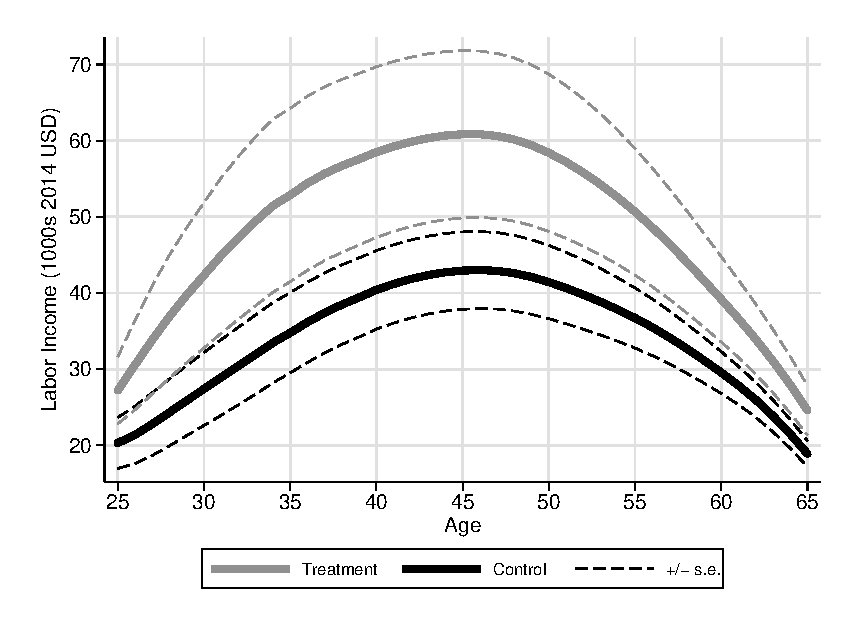
\includegraphics[width=\textwidth]{output/labor_25-60_male_2}
\end{subfigure}%
\begin{subfigure}[h]{0.35\textwidth}
		\centering
		\caption{Males, Based on Lagged Labor Income} 
		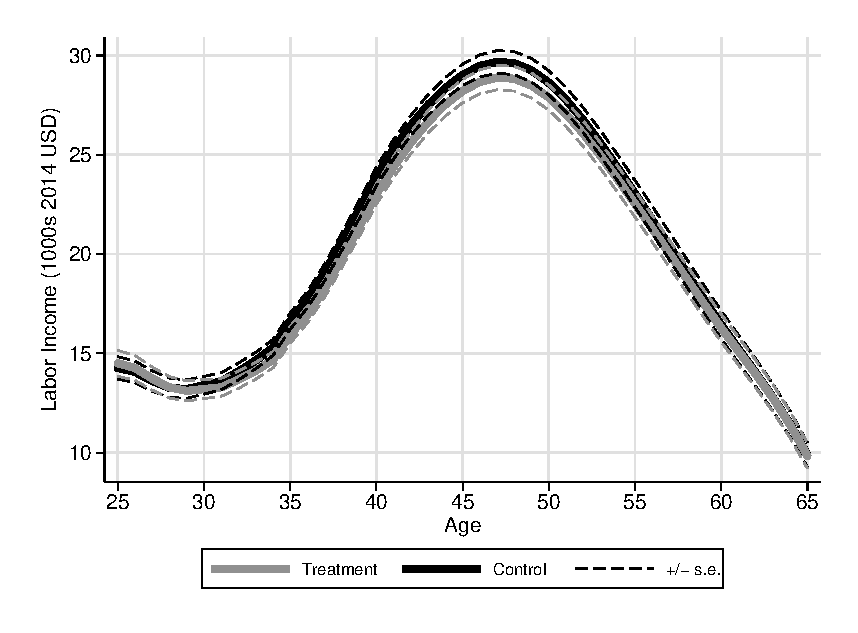
\includegraphics[width=\textwidth]{output/labor_25-60_male_3}
\end{subfigure}
\begin{subfigure}[h]{0.35\textwidth}
		\centering
		\caption{Females, Based on PIAT and Education} 
		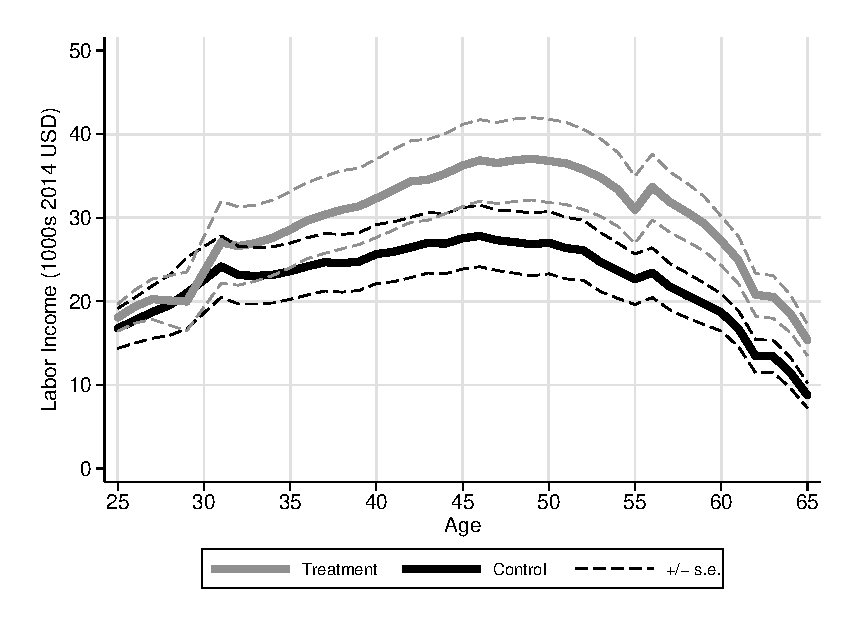
\includegraphics[width=\textwidth]{output/labor_25-60_female_2}
\end{subfigure}%
\begin{subfigure}[h]{0.35\textwidth}
		\centering
		\caption{Females, Based on Lagged Labor Income}
		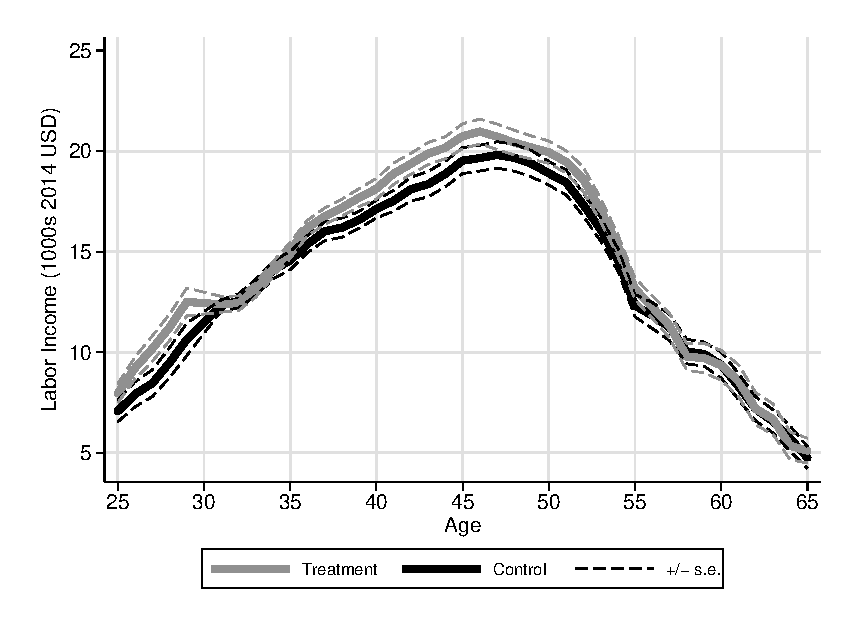
\includegraphics[width=\textwidth]{output/labor_25-60_female_3}
\end{subfigure}
\footnotesize \justify
Note: Panels (a) and (b) displays the forecast life-cycle labor income profiles for ABC/CARE males by treatment status, analogous to the forecasts in Figure~\ref{fig:labor-income-profiles} but using either PIAT (5-7) and years of education as predictors or lagged labor income. Figure~\ref{fig:labor-income-profiles} uses PIAT (5-7), years of education as predictors, and lagged labor income. Panels (c) and (d) are analogous to (a) and (b) for females.
\end{sidewaysfigure}

\pagebreak


%References
\singlespace
\bibliographystyle{chicago}
\bibliography{heckman}

\end{document}
